\documentclass[journal]{vgtc}                % final (journal style)
% \documentclass[review,journal]{vgtc}         % review (journal style)
%\documentclass[widereview]{vgtc}             % wide-spaced review
% \documentclass[preprint,journal]{vgtc}       % preprint (journal style)

% This is eysa's macro file
\usepackage[usenames,dvipsnames]{xcolor}
\usepackage{subfigure}

\usepackage{pifont}% http://ctan.org/pkg/pifont
\newcommand{\cmark}{\textcolor{Green}{\ding{51}}}%
\newcommand{\xmark}{\textcolor{red}{\ding{55}}}%

\newcommand{\eysa}[1]{\textcolor{Mulberry}{e: #1}}
\newcommand{\laura}[1]{\textcolor{blue}{l: #1}}
\newcommand{\sara}[1]{\textcolor{red}{s: #1}}
\newcommand{\amogh}[1]{\textcolor{green}{a: #1}}

%% Uncomment one of the lines above depending on where your paper is
%% in the conference process. ``review'' and ``widereview'' are for review
%% submission, ``preprint'' is for pre-publication, and the final version
%% doesn't use a specific qualifier.

%% Please use one of the ``review'' options in combination with the
%% assigned online id (see below) ONLY if your paper uses a double blind
%% review process. Some conferences, like IEEE Vis and InfoVis, have NOT
%% in the past.

%% Please note that the use of figures other than the optional teaser is not permitted on the first page
%% of the journal version.  Figures should begin on the second page and be
%% in CMYK or Grey scale format, otherwise, colour shifting may occur
%% during the printing process.  Papers submitted with figures other than the optional teaser on the
%% first page will be refused. Also, the teaser figure should only have the
%% width of the abstract as the template enforces it.

%% These few lines make a distinction between latex and pdflatex calls and they
%% bring in essential packages for graphics and font handling.
%% Note that due to the \DeclareGraphicsExtensions{} call it is no longer necessary
%% to provide the the path and extension of a graphics file:
%% 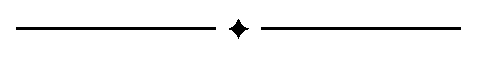
\includegraphics{diamondrule} is completely sufficient.
%%
\ifpdf%                                % if we use pdflatex
  \pdfoutput=1\relax                   % create PDFs from pdfLaTeX
  \pdfcompresslevel=9                  % PDF Compression
  \pdfoptionpdfminorversion=7          % create PDF 1.7
  \ExecuteOptions{pdftex}
  \usepackage{graphicx}                % allow us to embed graphics files
  \DeclareGraphicsExtensions{.pdf,.png,.jpg,.jpeg} % for pdflatex we expect .pdf, .png, or .jpg files
\else%                                 % else we use pure latex
  \ExecuteOptions{dvips}
  \usepackage{graphicx}                % allow us to embed graphics files
  \DeclareGraphicsExtensions{.eps}     % for pure latex we expect eps files
\fi%

%% it is recomended to use ``\autoref{sec:bla}'' instead of ``Fig.~\ref{sec:bla}''
\graphicspath{{figures/}{pictures/}{images/}{./}} % where to search for the images

\usepackage{microtype}                 % use micro-typography (slightly more compact, better to read)
\PassOptionsToPackage{warn}{textcomp}  % to address font issues with \textrightarrow
\usepackage{textcomp}                  % use better special symbols
\usepackage{mathptmx}                  % use matching math font
\usepackage{times}                     % we use Times as the main font
\renewcommand*\ttdefault{txtt}         % a nicer typewriter font
\usepackage{cite}                      % needed to automatically sort the references
\usepackage{tabu}                      % only used for the table example
\usepackage{booktabs}                  % only used for the table example
%% We encourage the use of mathptmx for consistent usage of times font
%% throughout the proceedings. However, if you encounter conflicts
%% with other math-related packages, you may want to disable it.

%% In preprint mode you may define your own headline.
%\preprinttext{To appear in IEEE Transactions on Visualization and Computer Graphics.}

%% If you are submitting a paper to a conference for review with a double
%% blind reviewing process, please replace the value ``0'' below with your
%% OnlineID. Otherwise, you may safely leave it at ``0''.
\onlineid{0}

%% Paper title.
\title{Spotify Visualization: Visualizing Music Listening History}
%% This is how authors are specified in the journal style

%% indicate IEEE Member or Student Member in form indicated below
\author{Sara Di Bartolomeo, Eysa Lee, Amogh Pradeep, Laura South}
\authorfooter{
%% insert punctuation at end of each item
\item
 Sara Di Bartolomeo, Eysa Lee, Amogh Pradeep, and Laura South are with Northeastern University. E-mail: \{dibartolomeo.s\,$|$\,lee.ey\,$|$\,pradeep.am\,$|$\,south.l\}@husky.neu.edu.
}

%other entries to be set up for journal
\shortauthortitle{Di Bartolomeo \MakeLowercase{\textit{et al.}}: My Week in Music: Visualizing Music Listening History}
%\shortauthortitle{Firstauthor \MakeLowercase{\textit{et al.}}: Paper Title}

%% Abstract section.
\abstract{\eysa{todo}%
} % end of abstract

%% Keywords that describe your work. Will show as 'Index Terms' in journal
%% please capitalize first letter and insert punctuation after last keyword
\keywords{personalized, music, history, stacked area chart\eysa{I'm not super familiar with visualization keywords... plaese help}}

%% ACM Computing Classification System (CCS). 
%% See <http://www.acm.org/class/1998/> for details.
%% The ``\CCScat'' command takes four arguments.

% \CCScatlist{ % not used in journal version
%  \CCScat{K.6.1}{Management of Computing and Information Systems}%
% {Project and People Management}{Life Cycle};
%  \CCScat{K.7.m}{The Computing Profession}{Miscellaneous}{Ethics}
% }

%% Uncomment below to include a teaser figure.
\teaser{
  \centering
  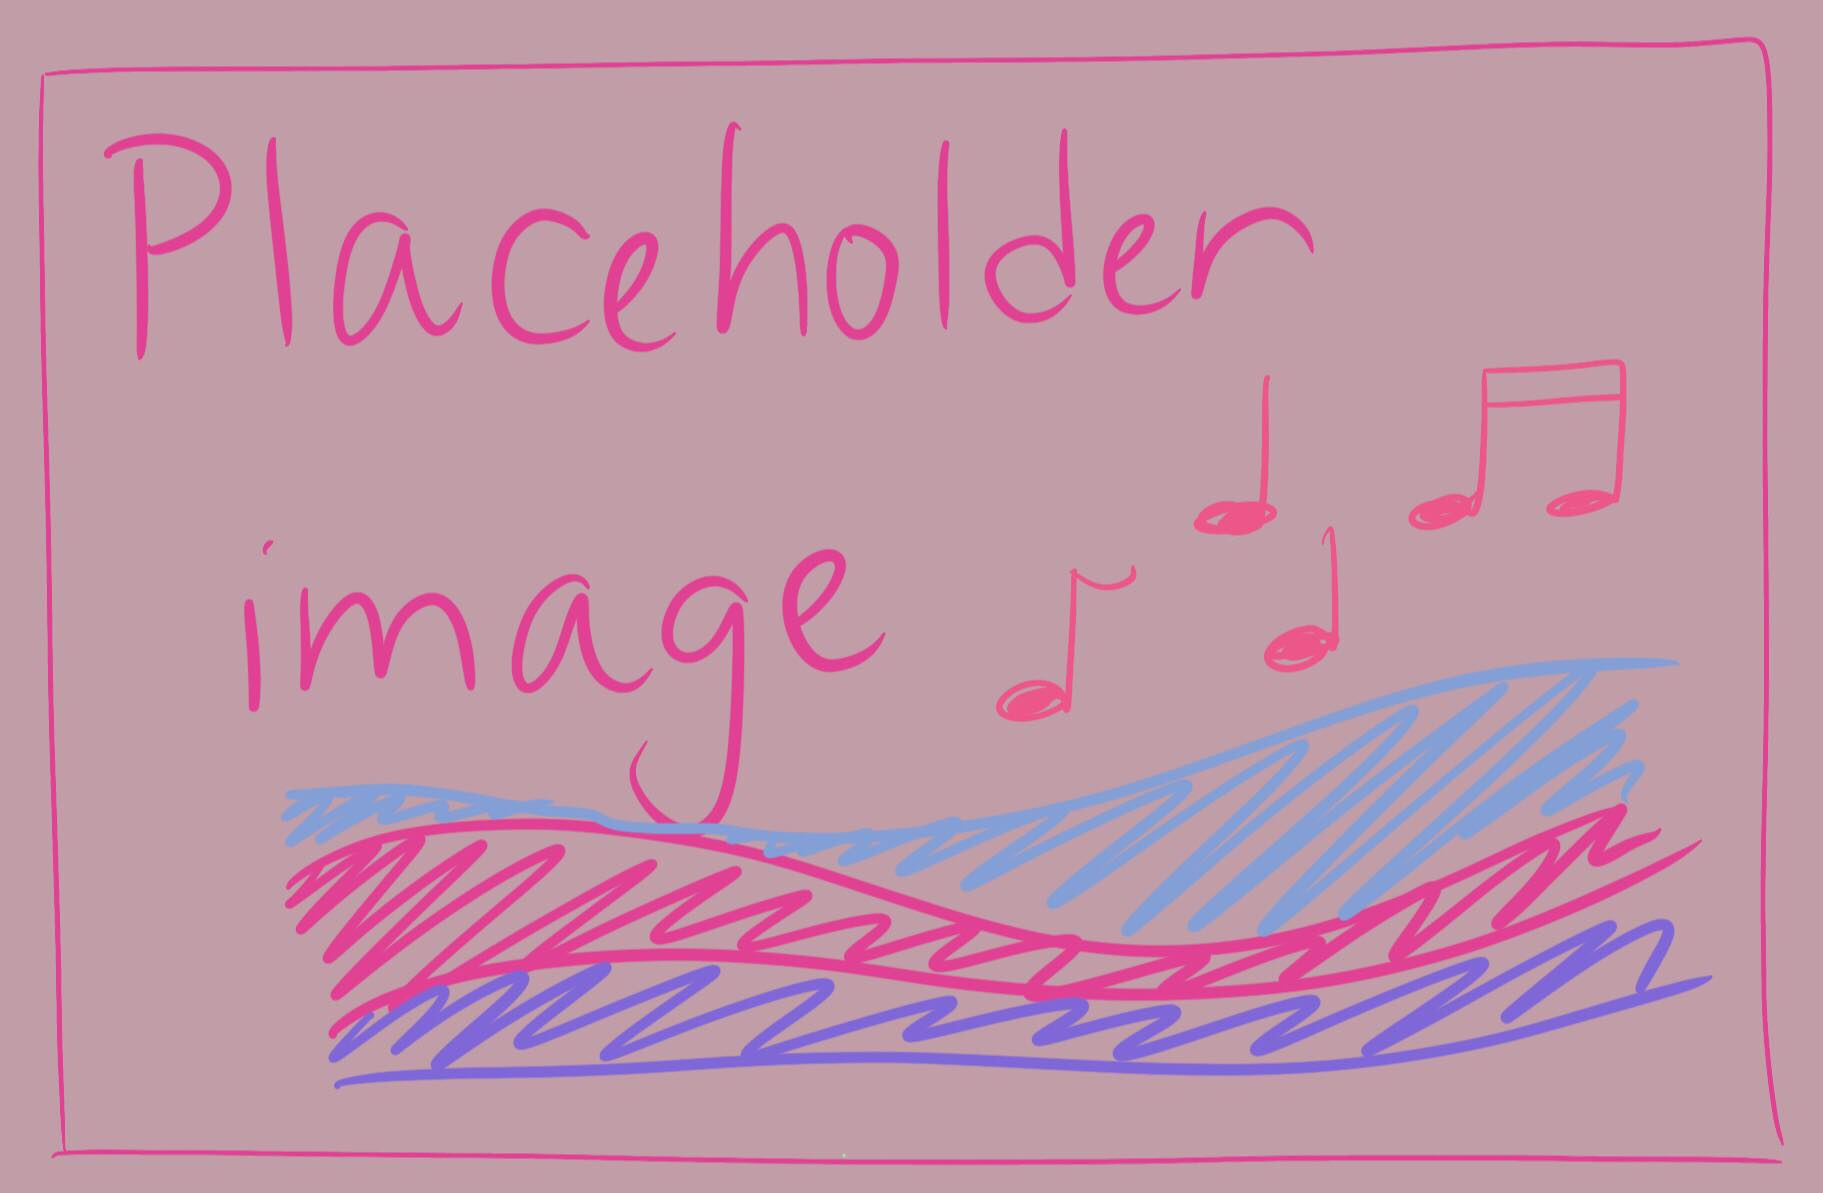
\includegraphics[width=0.75\linewidth]{placeholder_image}
  \caption{A week in music: \eysa{Tentative screenshot of our thing}.}
	\label{fig:teaser}
}

%% Uncomment below to disable the manuscript note
%\renewcommand{\manuscriptnotetxt}{}

%% Copyright space is enabled by default as required by guidelines.
%% It is disabled by the 'review' option or via the following command:
\nocopyrightspace

\vgtcinsertpkg

%%%%%%%%%%%%%%%%%%%%%%%%%%%%%%%%%%%%%%%%%%%%%%%%%%%%%%%%%%%%%%%%
%%%%%%%%%%%%%%%%%%%%%% START OF THE PAPER %%%%%%%%%%%%%%%%%%%%%%
%%%%%%%%%%%%%%%%%%%%%%%%%%%%%%%%%%%%%%%%%%%%%%%%%%%%%%%%%%%%%%%%%

\begin{document}

%% The ``\maketitle'' command must be the first command after the
%% ``\begin{document}'' command. It prepares and prints the title block.

%% the only exception to this rule is the \firstsection command
\firstsection{Introduction}

\maketitle

Spotify is one of the most popular music streaming service, with 207 million monthly active users in 2018. The app does not currently provide users with a way to view their personal listening history despite the popularity of its annual end of year visualization, which provides users a high-level overview of a their listening habits for the year. Several third-party apps allow users to see their personal listening data, but none fully utilize the power of data visualizations to convey information. In this work we create an interactive data visualization using information available from the Spotify API to help users better understand their personal listening patterns.

\section{Related Works}
Many applications exist to visualization a user's Spotify listening history, with usages and data being displayed varying. We will consider the related works as two broad categories: (1) Spotify's official end of year visualization and (2) third-party applications.

\subsection{Spotify's End of Year Visualization}

While generally Spotify does not provide user's with a way to visualize their personal listening history, at the end of each year Spotify releases a visualization `summarizing' a user's listening history for the past year\cite{Spo18}.

This visual summary has gone by different names over the years, such as \emph{SpotifyWrapped} and \emph{Year in Review}, but the purpose of the visualization has remained fairly consistent. It focuses on giving users an overview of their year by displaying aggregated data, such as total minutes listened, top tracks, top artists, and top genre. Additionally, it only displays data from a fixed range of time (January to October) and only displays a fixed number of tracks and artists. While this accomplishes the purpose of giving a year summary for a user, it does not provide users much freedom in exploring their data. This visualization has the additional drawback of only being available for a limited amount of time each year.

\subsection{Third-party Applications}

Many third-party services exist to utilize the data available from using a music streaming service. One of the more popular services is Last.fm, which gives users an interface to explore their data upon connecting to their streaming service. This has spawned applications such as \cite{Pre08,Dan12}, which use Last.fm's API to allow users to explore their personal data.
These services, however, either require a lot of upfront effort from the user to use their service (such as registering an account)\eysa{what's a better way to phrase this?} or provide \emph{too much} data and can be difficult for a user to process.

Another popular class of third-party applications are simply scripts written by curious programmers, such as \cite{Boe16}. It is hardly surprising that many casual programmers, noticing the abundance of data and lack of existing popular visualization, whip up scripts visualizing their personal data and make the code available for others. This class of applications suffers from similar drawbacks to services using Last.fm. These mostly lack web interfaces, which results in work for a user to download and figure out how to run scripts. Additionally, these applications mostly try to visualize as much as possible, which can be an overwhelming amount of data for a user.

\section{Design Process}

\subsection{Task Analysis}

\begin{table}[tb]
  \caption{Summary of User Interviews: Columns are marked `\cmark' if the user indicated interest, `\xmark' if the user indicated no interest, and `-' if the user gave no indication of interest or disinterest during the interview.}
  \label{tab:interviews}
  \scriptsize%
    \centering%
  \begin{tabu}{%
    r%
    *{7}{c}%
    *{2}{r}%
    }
  \toprule
    & \rotatebox{90}{Personal Stats} \rotatebox{90}{(e.g. Top Tracks)} & \rotatebox{90}{Comparing data} \rotatebox{90}{with others} & \rotatebox{90}{Change over time} & \rotatebox{90}{`Interesting' Stats} \\
  \midrule
  Megan & \cmark & \cmark & \cmark & \cmark \\
  Matthew & \cmark & \cmark & \cmark & \cmark \\
  Giorgio & \cmark & \cmark & \xmark & \xmark \\
  Akshar & \cmark & \xmark & \cmark & \cmark \\
  Sarah & \cmark & \xmark & \cmark & - \\
  Tanay & \xmark & \cmark & \cmark & - \\
  Ali & \xmark & \cmark & - & - \\
  Connor & \xmark & \cmark & - & - \\
  Yash & \xmark & - & - & \cmark \\
  \midrule
  \textbf{Sums (\cmark:\xmark)} & \textbf{5:4} & \textbf{6:2} & \textbf{5:1} & \textbf{4:1} \\
  \bottomrule
  \end{tabu}%
\end{table}


In order to determine tasks to prioritize in our design, we interviewed potential users of our visualization. Nine short interviews with people of varying listening habits were conducted to prevent overfitting to a single person's preferences. The interviews consisted of asking about (1) listening habits, (2) previous interactions with personalized music history visualizations, if at all, (3) data they're interested in visualizing, and (4) data they're not interested in being visualized. Summaries of responses are reported in \autoref{tab:interviews}.

From our interviews, we determined our domain goals to be the following:
\begin{enumerate}
  \item View daily listening history split by genre
  \item View recent top artists/tracks
  \item Compare listening history between users
\end{enumerate}

\eysa{todo: add discussion about these domain goals}

\subsection{Data Acquisition and Exploratory Analysis}
Data Acquisition and Exploratory Analysis Outline:
\begin{itemize}
  \item Tested fetching data using Spotify API, generally didn't find bad data
  \item Discovered getting breakdown of music by day or hour requires retrieving many batches of last played and looking at timestamps; limitations on the granularity our visualization can display
\end{itemize}

\section{Design}

\subsection{Mockup}
\begin{figure*}
\centering
\mbox{
  \subfigure[Static mockup.\label{fig:static_mockup}]{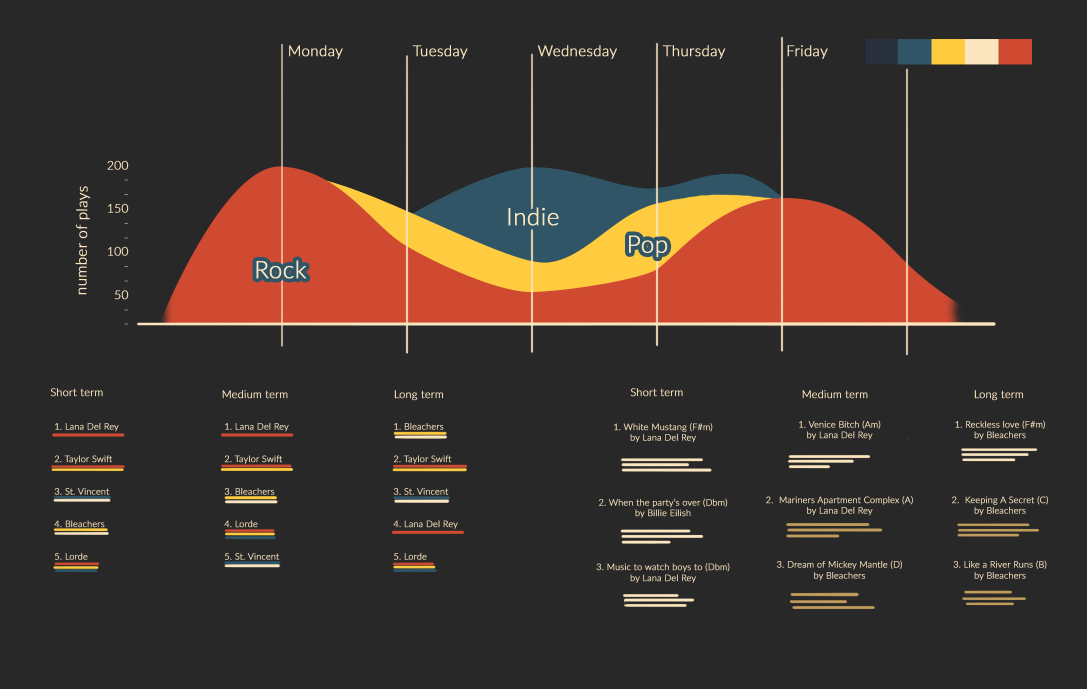
\includegraphics[width=0.45\textwidth]{mockup}}\quad
  \subfigure[Genre interaction.\label{fig:genre_interaction}]{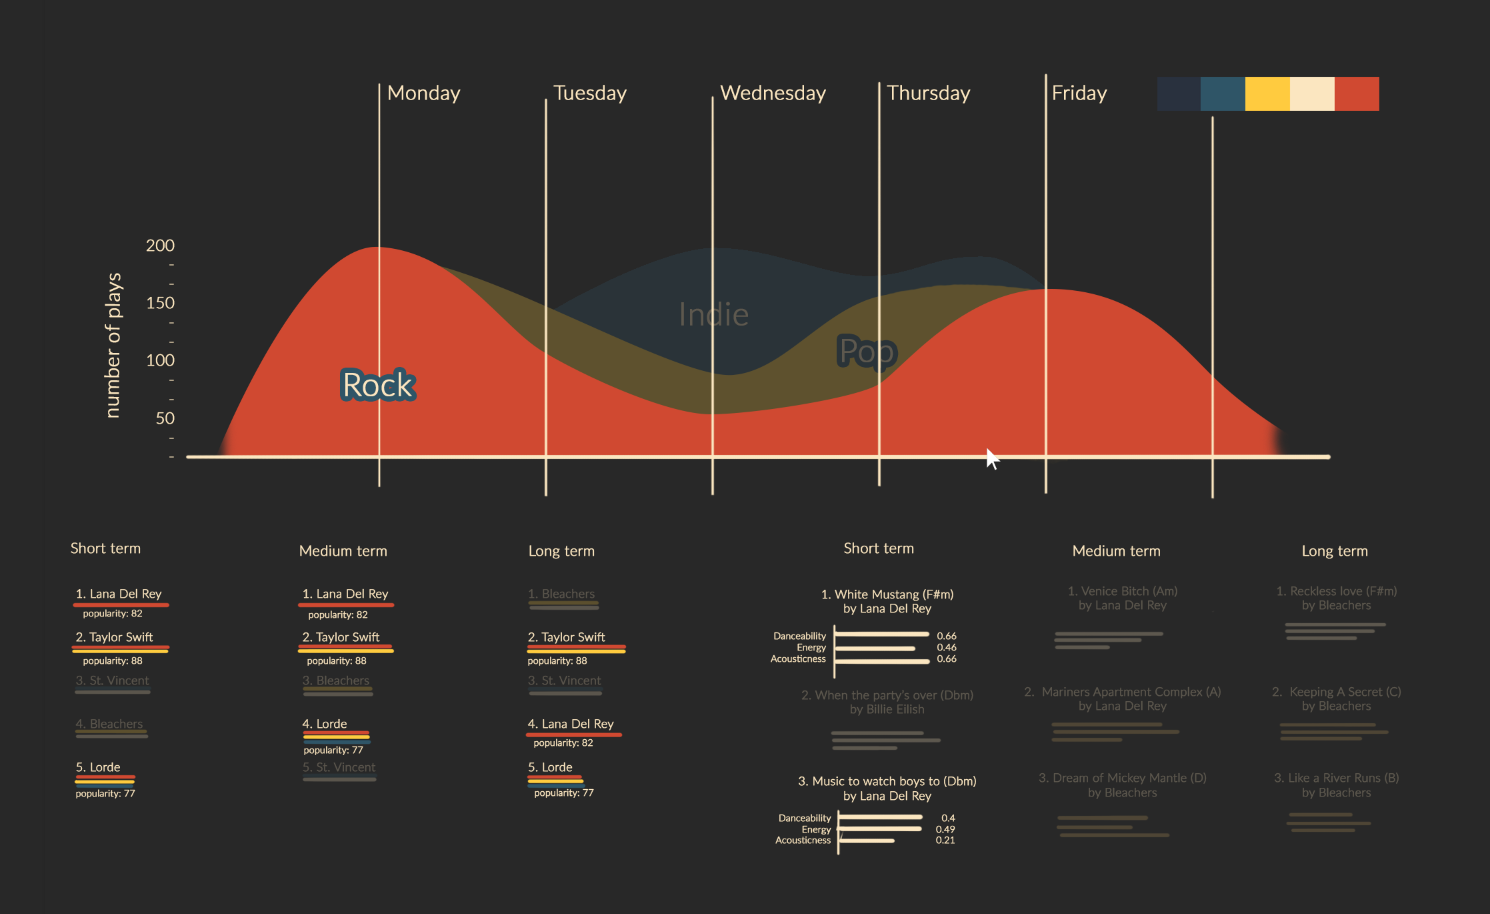
\includegraphics[width=0.45\textwidth]{genre_interaction}}
}
\\
\mbox{
  \subfigure[Artist interaction.\label{fig:artist_interaction}]{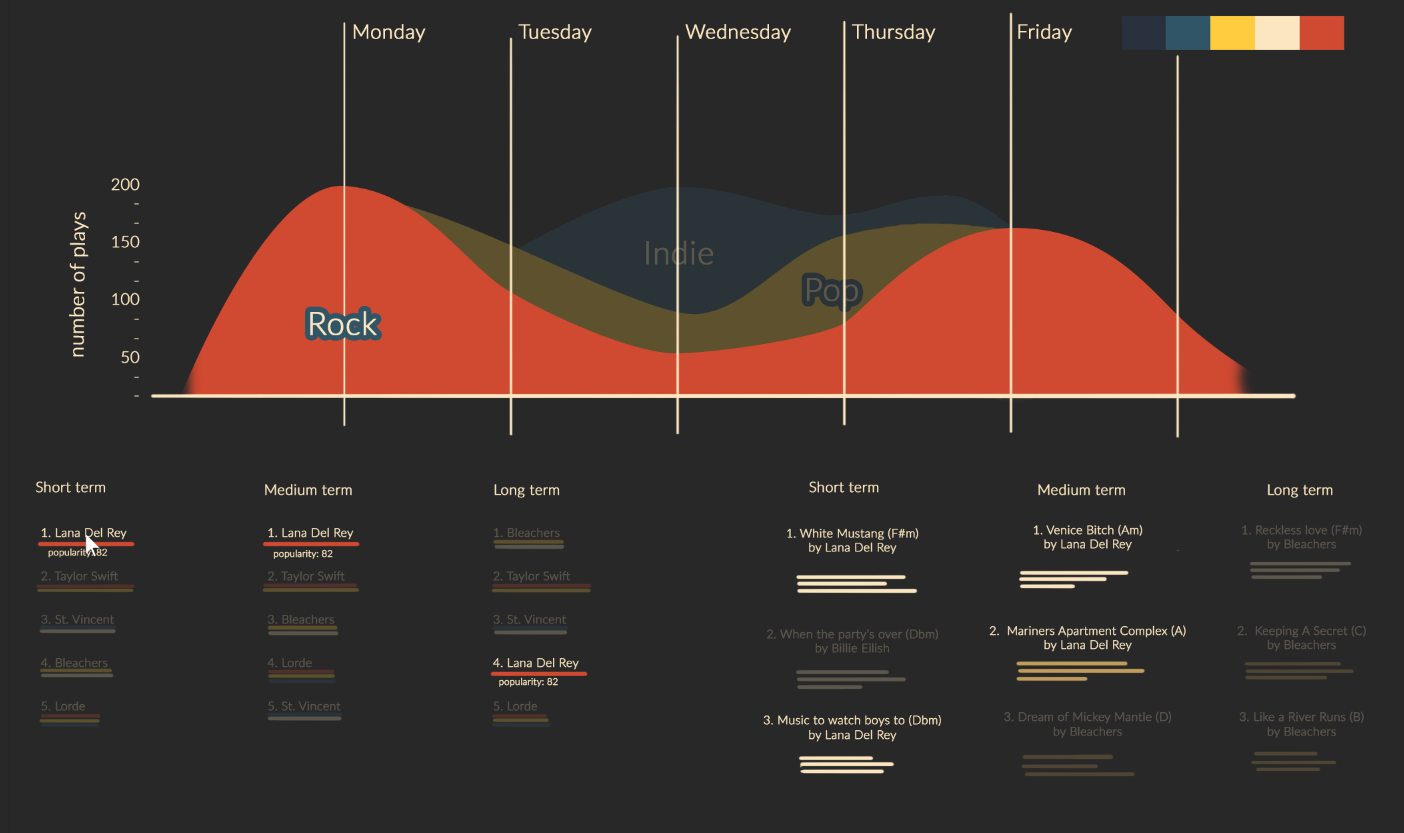
\includegraphics[width=0.45\textwidth]{artist_interaction}}\quad
  \subfigure[Track interaction.\label{fig:track_interaction}]{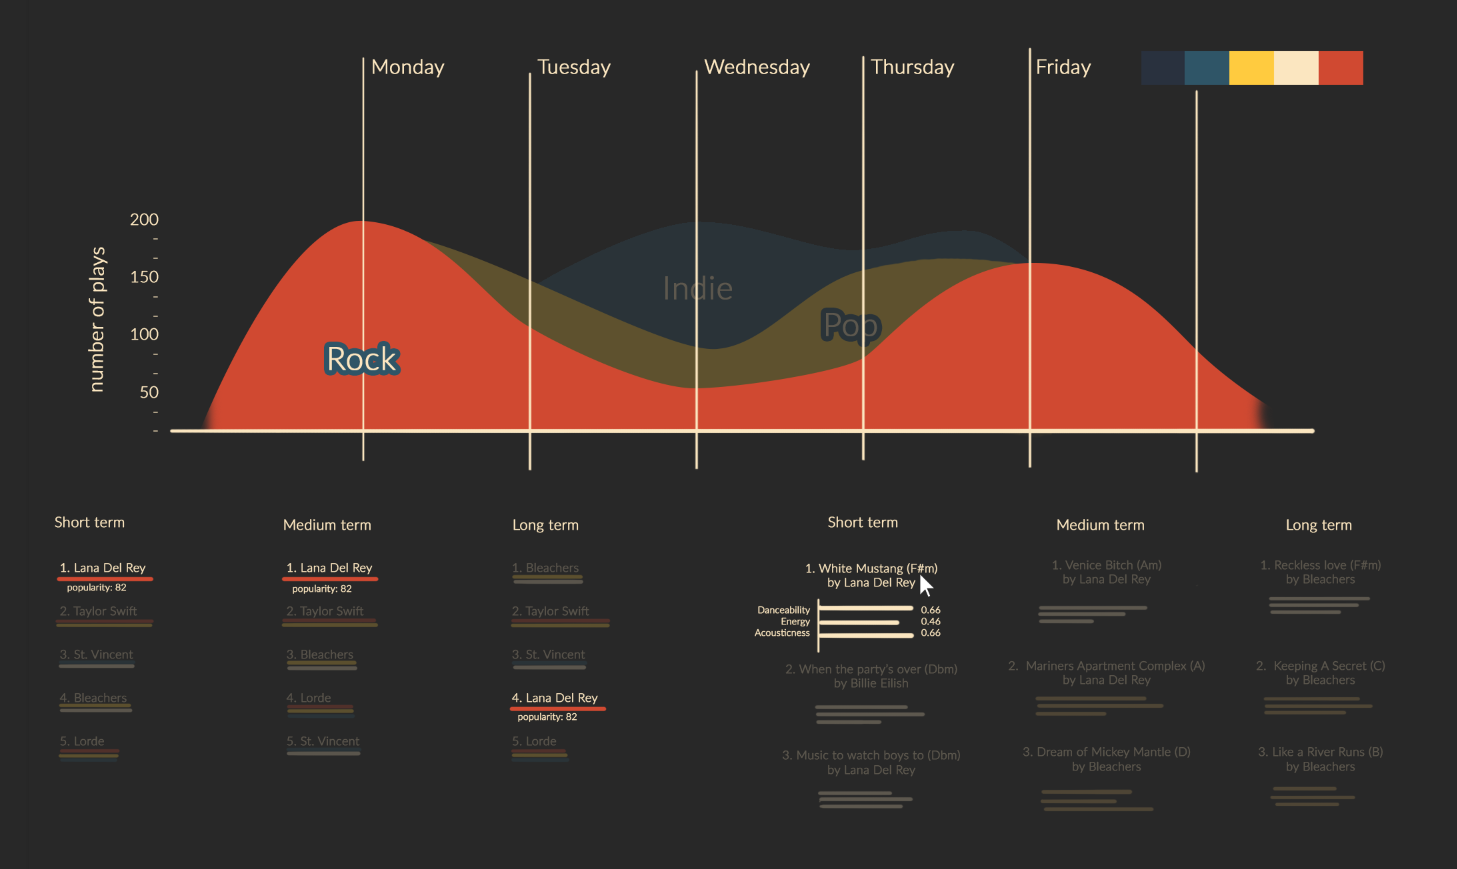
\includegraphics[width=0.45\textwidth]{track_interaction}}
}
\caption{Primary interactions: Hovering over different sections in the visualization highlights and connects related data between the stacked area chart and the two lists.}
\label{fig:interactions}
\end{figure*}

Design outline:
\begin{itemize}
  \item Captured our domain goals in the final sketch of what we wanted\eysa{can add the final sketches}. Interactions with these sketches can be seen in \autoref{fig:interactions}
  \item Talk about how the sketch accomplishes our domain goals
  \begin{itemize}
    \item We prioritized the first two domain goals because user interviews indicated people cared more about personal data
  \end{itemize}
  \item Changes between sketch and implementation. Was there anything we changed based on classmates testing our preliminary design
  \item Implementation (screenshot and description)
\end{itemize}

\subsection{Preliminary Usability Testing}
Outline:
\begin{itemize}
  \item Explain how we conducted our usability tests (Introduced our project and asked users to play around with the visualization; asked users if they could identify what particular things were supposed to represent)
  \item Pros: color scheme, nice to look at
  \item Cons: Hard to see when artists/tracks are bolded (doesn't stand out much); columns are not labled; no title to indicate if the visualization is a prediction or history of music listening; stream graph and lists don't fit on the screen together
  \item How to visualize genres in stream graph without overloading it?
\end{itemize}

\begin{figure*}
\centering
\mbox{
  \subfigure[Static mockup.\label{fig:static_prelim}]{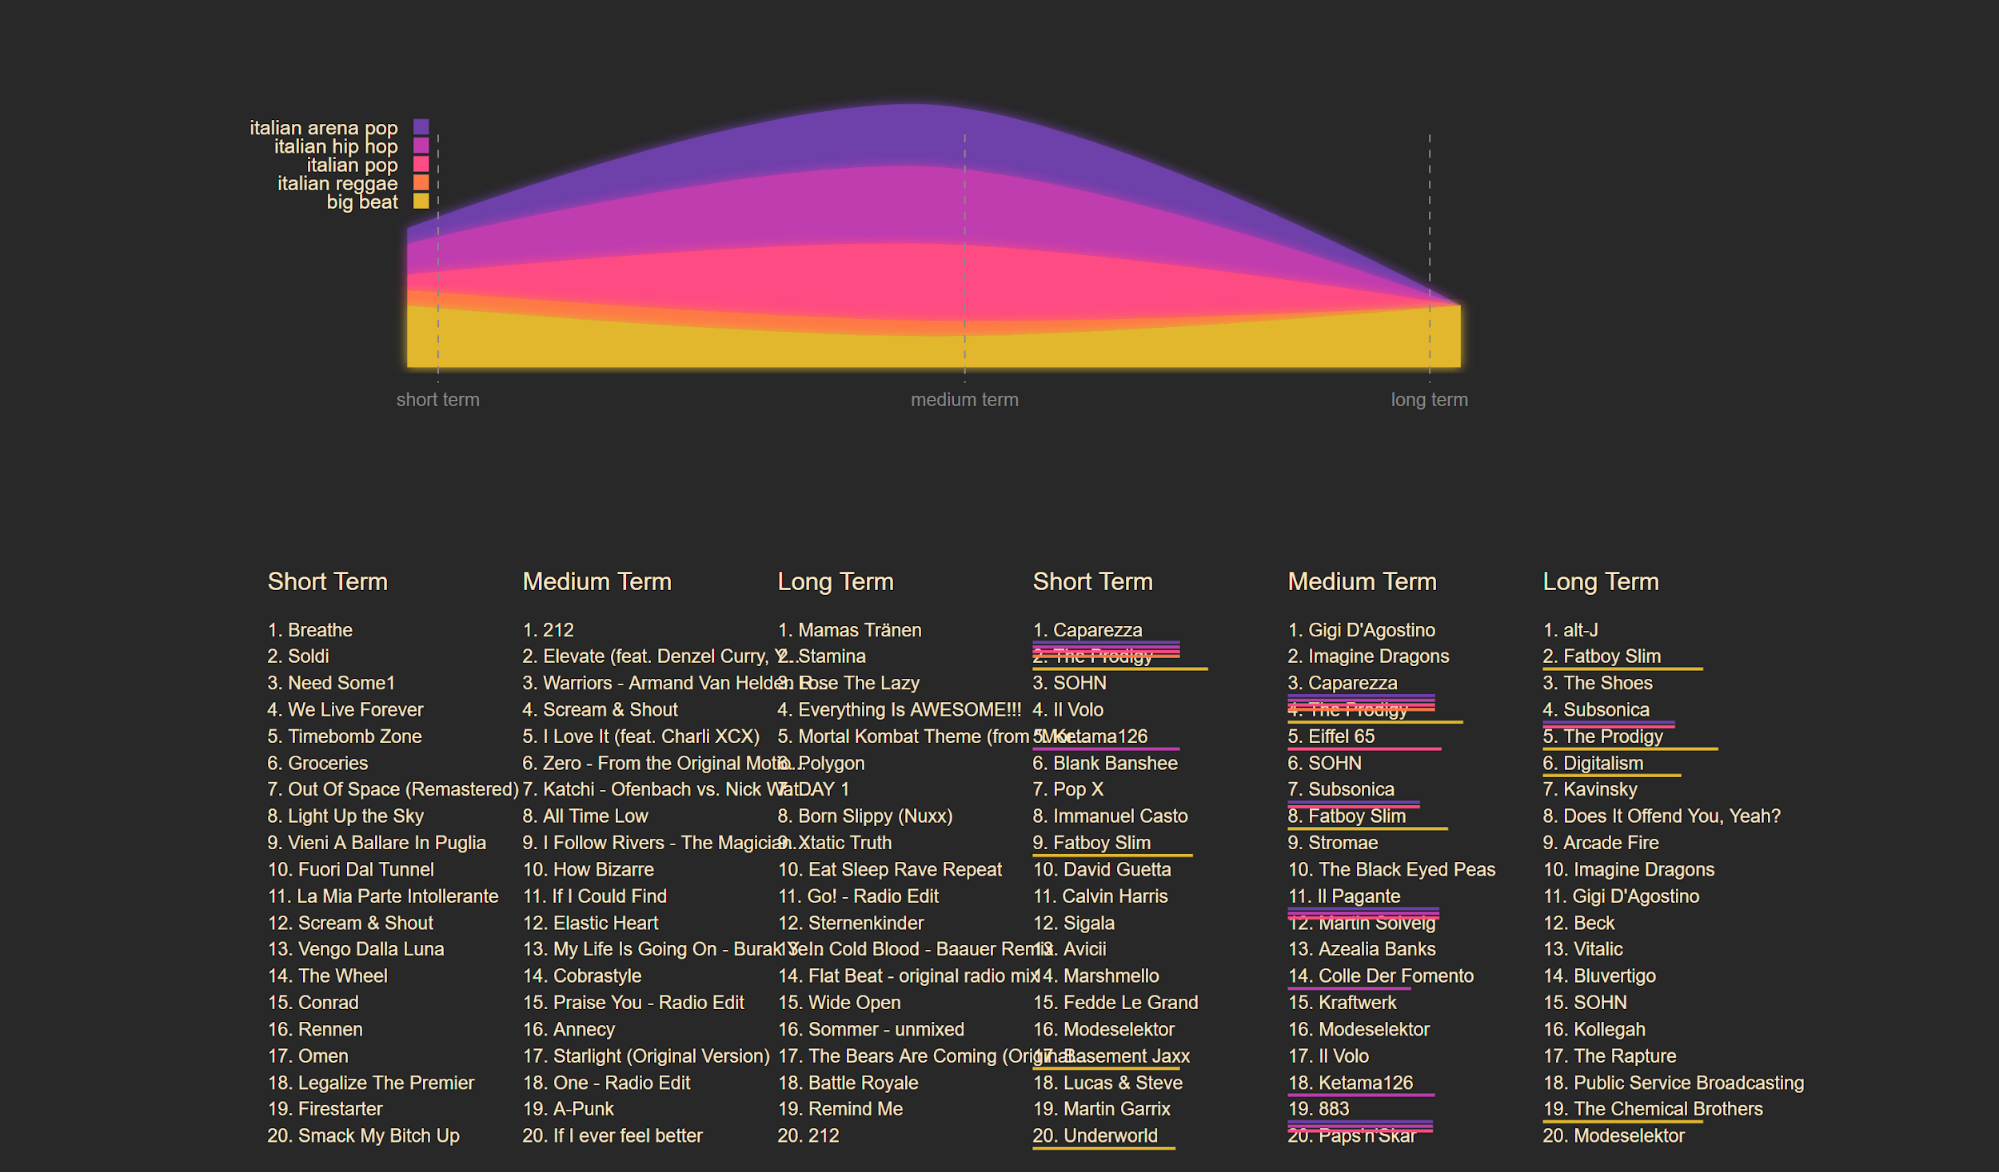
\includegraphics[width=0.45\textwidth]{ms4_static}}\quad
  \subfigure[Genre interaction.\label{fig:genre_prelim}]{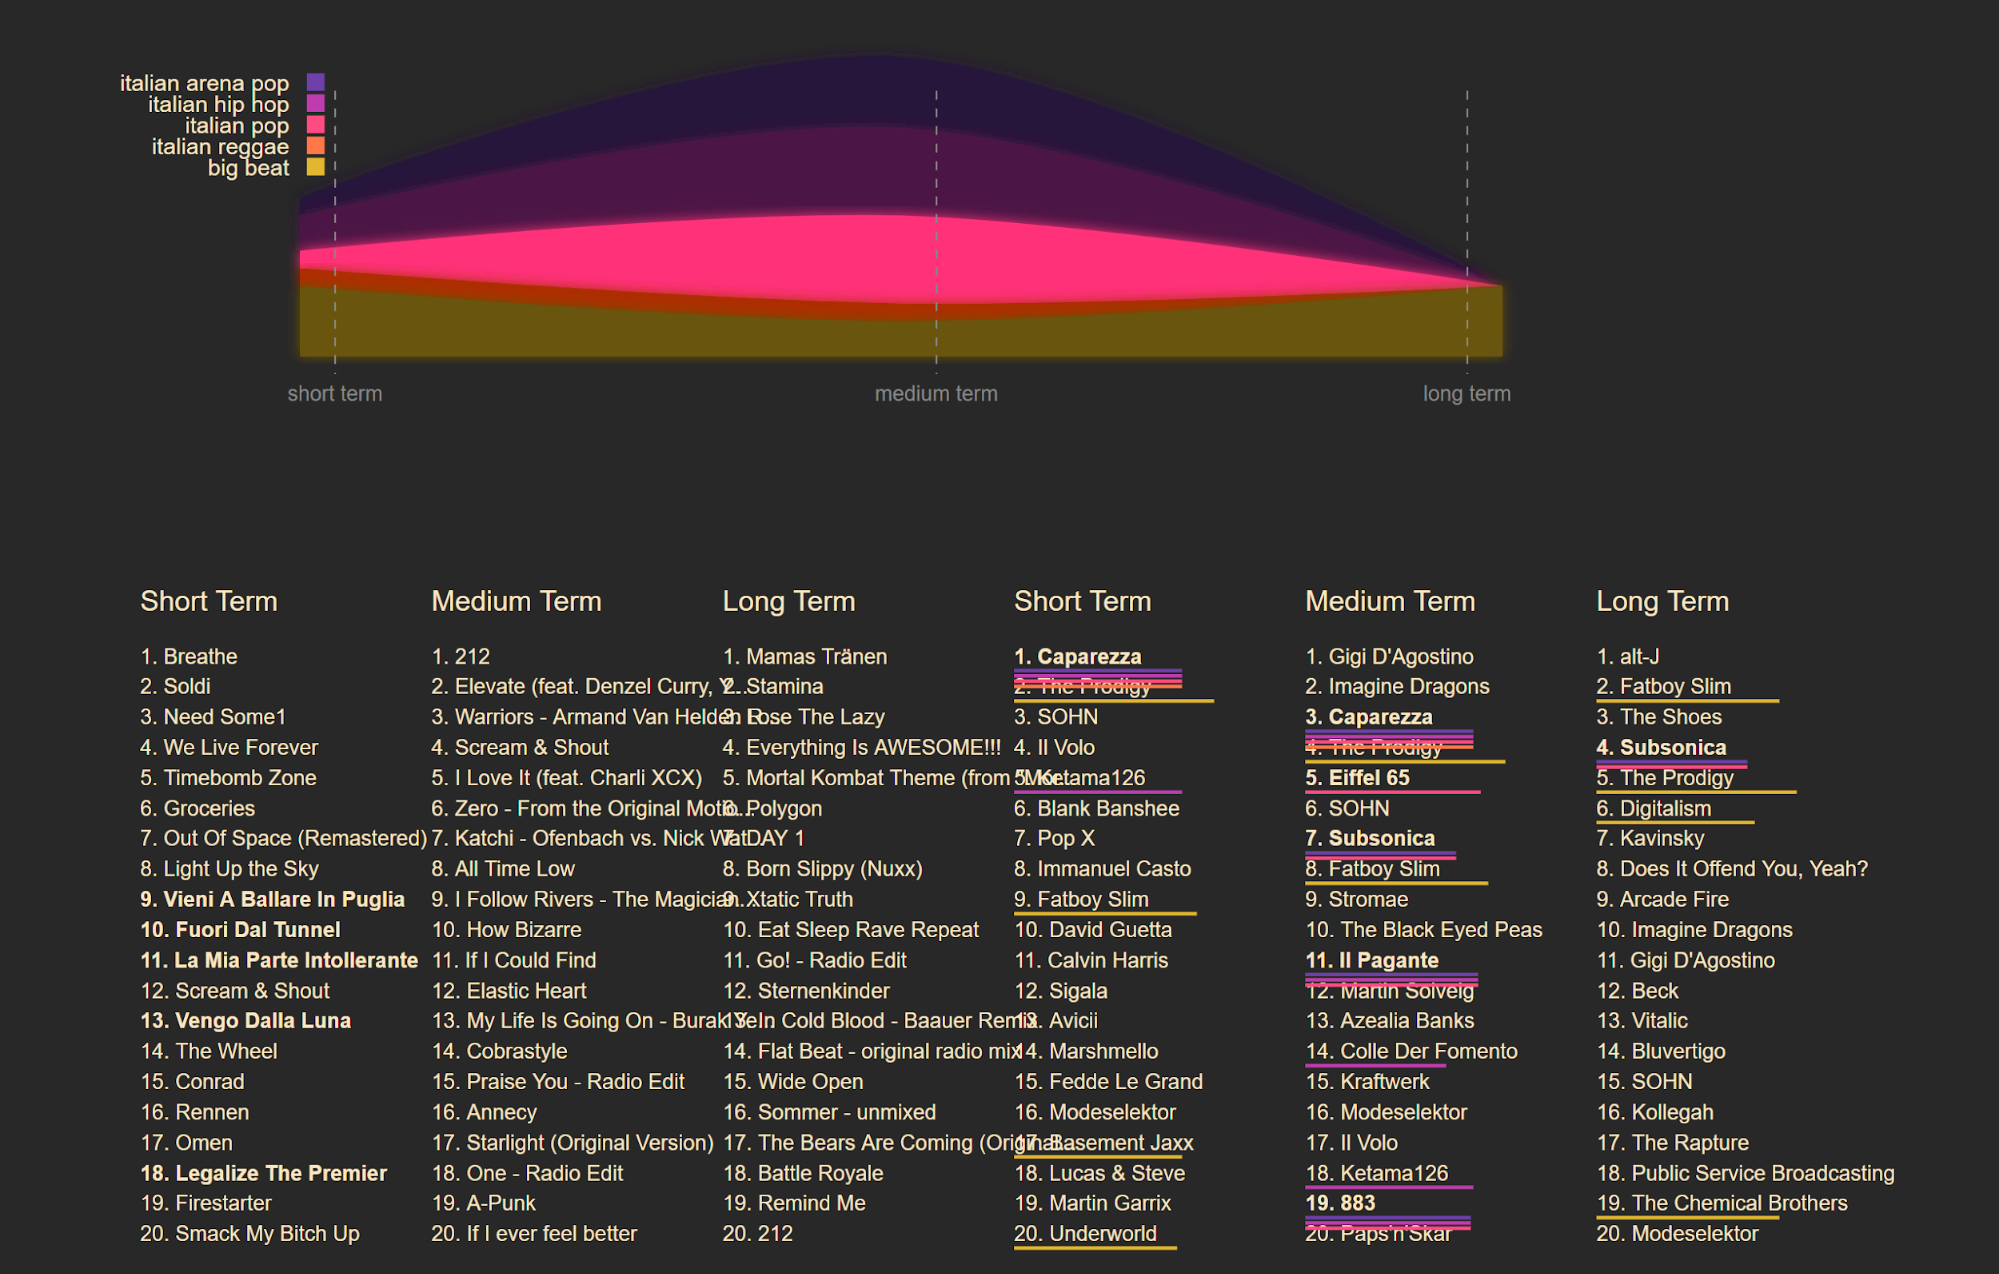
\includegraphics[width=0.45\textwidth]{ms4_genre}}
}
\\
\mbox{
  \subfigure[Artist interaction.\label{fig:artist_prelim}]{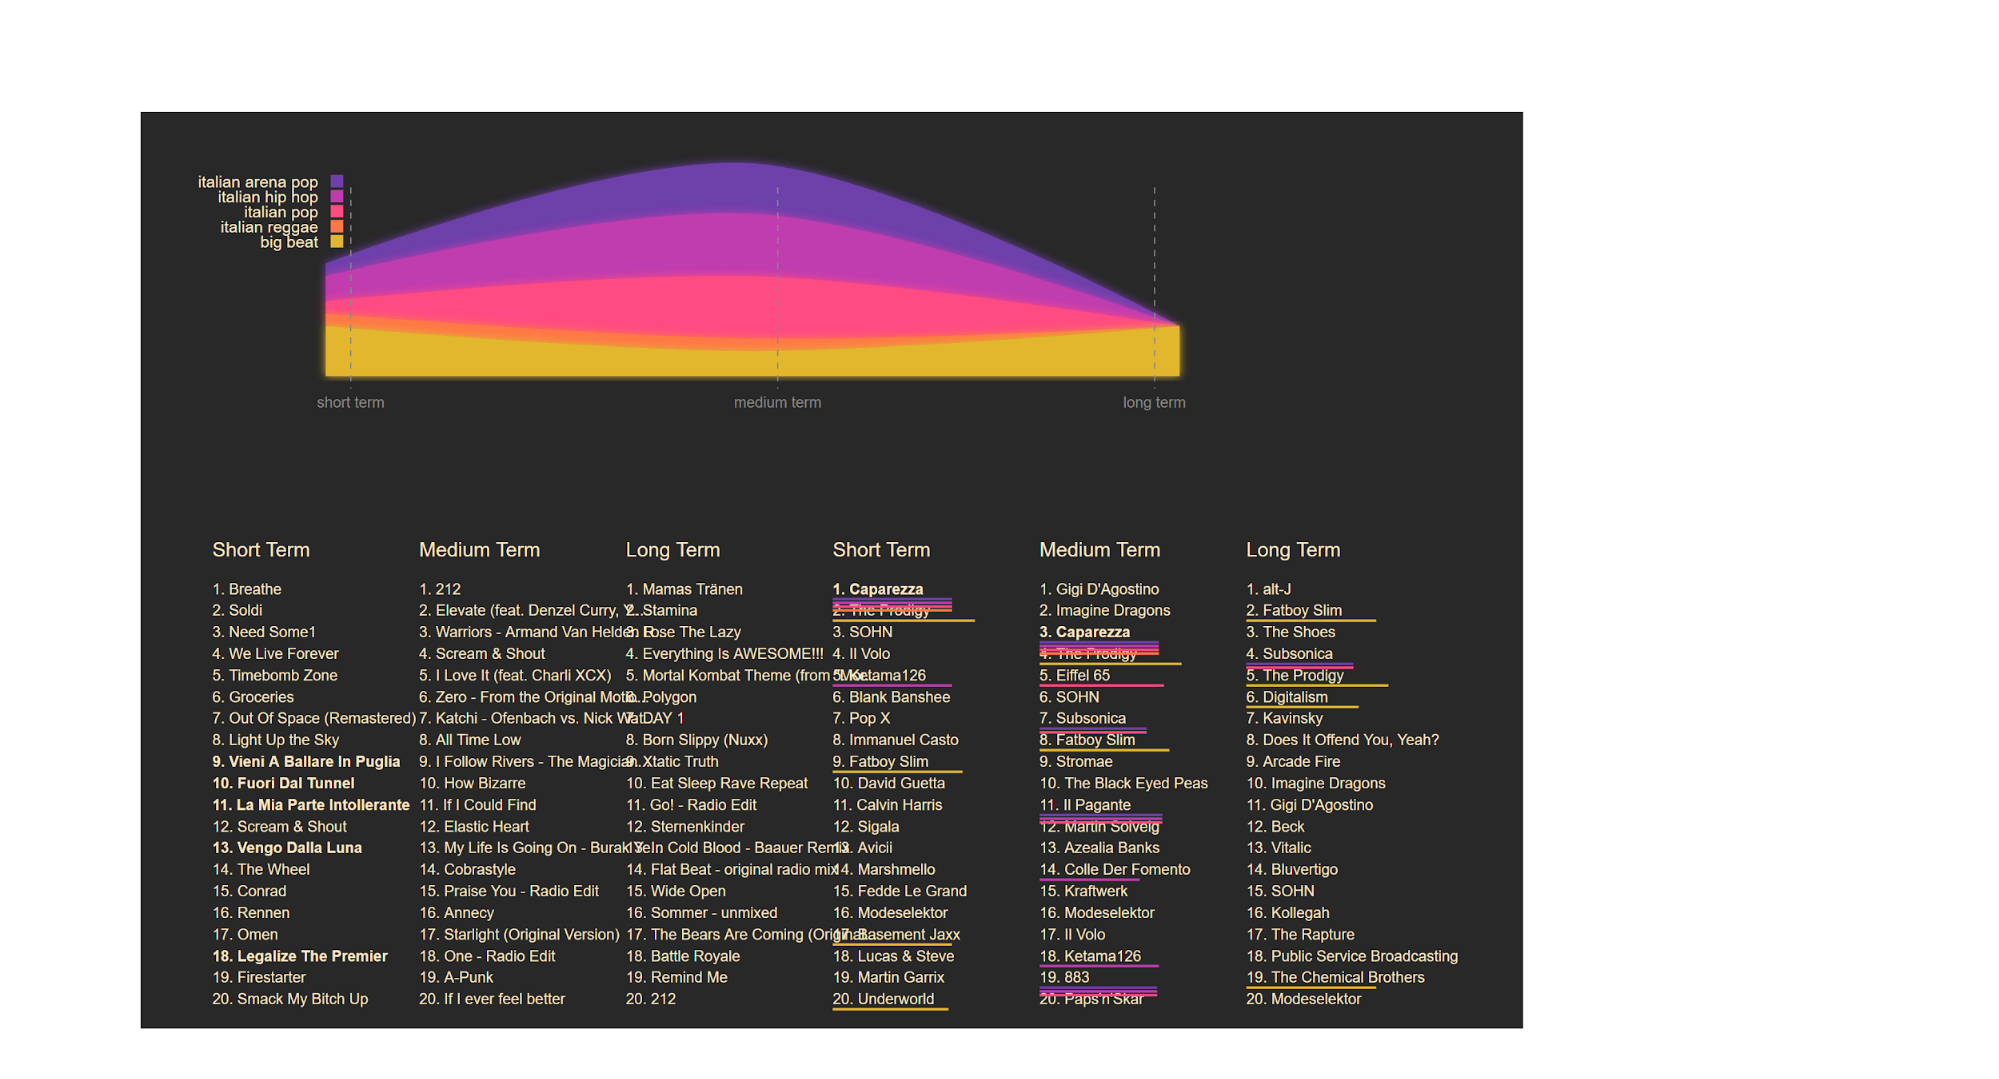
\includegraphics[width=0.45\textwidth]{ms4_artist}}\quad
  \subfigure[Track interaction.\label{fig:track_prelim}]{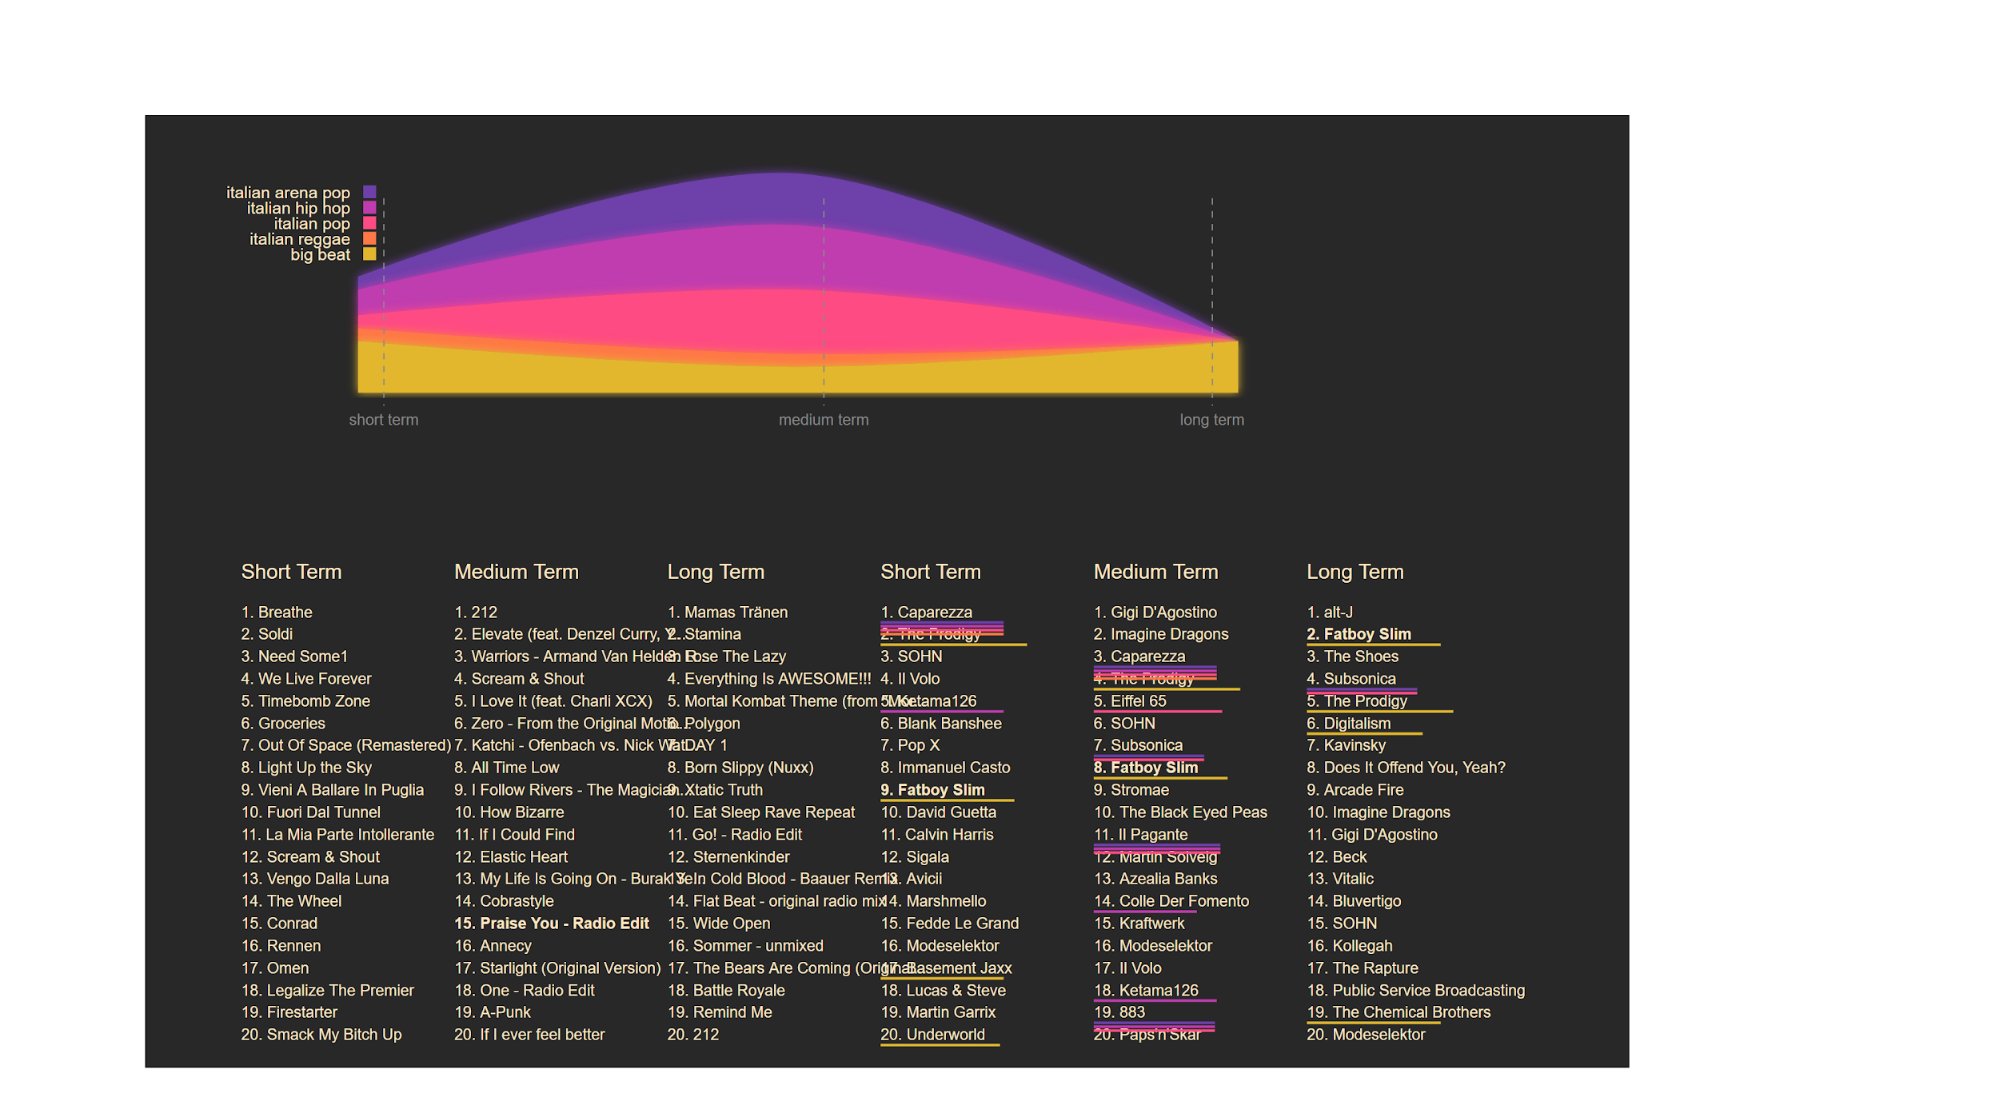
\includegraphics[width=0.45\textwidth]{ms4_track}}
}
\caption{Preliminary Design: State of the visualization during usability testing. Users found the visualization aesthetically pleasing but struggled with interpreting all of the information encoded in the design.}
\label{fig:prelim_design}
\end{figure*}

\subsection{Final Design}

Modifications based on usability testing:
\begin{itemize}
  \item Moved stream graph and track/artist columns horizontally; took advantage of most desktop screens being wider than taller and placed things on the side
  \item Added an "other" category for genre; not having an "other" category previously made for some stream graphs appearing to get smaller in mid ranges; compromise to not overload graph with too many colors but not lose the data
  \item Added titles to the track/artist columns
  \item Changed genre encodings on artist to circles; artists may have many genres associated with them, so this eliminates lines overflowing over other text
  \item Added fade/bolding across artist columns to better visualize relationships across columns
  \item Added description at the bottom to explain the visualization
  \item Added tooltip walkthrough to explain how the visualization works
\end{itemize}

Outline:
\begin{itemize}
  \item How did our final design change?
  \item Main aspects of the final design
\end{itemize}

\section{Discussion}

Discussion outline:
\begin{itemize}
  \item What was the response like?
  \item What were areas we wanted to explore but couldn't
  \item What could we improve?
  \item Usability testing:
  \begin{itemize}
    \item Early usability testing suggested users had difficulty discovering all of the features of the visualization.
  \end{itemize}
\end{itemize}

\section{Conclusion}

Future directions include:
\begin{itemize}
  \item Computing over the data
  \item How can we make it easier for people to compare?
  \begin{enumerate}
    \item Maybe change genre color scheme to be the same for each genre rather than same colors for each user?
  \end{enumerate}
\end{itemize}

%% if specified like this the section will be committed in review mode
\acknowledgments{
The authors wish to thank the Spring 2019 teaching staff of Michelle Borkin's CS 7250 class for their helpful comments and guidance.
}

%\bibliographystyle{abbrv}
\bibliographystyle{abbrv-doi}
%\bibliographystyle{abbrv-doi-narrow}
%\bibliographystyle{abbrv-doi-hyperref}
%\bibliographystyle{abbrv-doi-hyperref-narrow}

\bibliography{references}
\end{document}

